% Supplementary material, built by manuscript/build.sh alongside paper.pdf. The figure legends
% state the sample size, uncertainty definition and source table. Numerical values are checked
% by scripts/audit_manuscript.py against the committed result tables.
\documentclass[11pt]{article}

\usepackage[margin=1in]{geometry}
\usepackage{graphicx}
\usepackage{amsmath}
\usepackage{booktabs}
\usepackage{longtable}
\usepackage{caption}
\usepackage[colorlinks=true,allcolors=blue]{hyperref}

\captionsetup{labelfont=bf,font=small,justification=raggedright,singlelinecheck=false}
\renewcommand{\thefigure}{S\arabic{figure}}
\renewcommand{\thetable}{S\arabic{table}}
\setlength{\parskip}{0.4em}
\setlength{\parindent}{0pt}

\hypersetup{
  pdftitle={Supplementary material: Apparent sequence-model contribution depends strongly on
            negative-set construction: a calibration across 94 ENCODE eCLIP datasets},
  pdfauthor={Nirmalkumar Thirupallikrishnan Kesavan},
  pdfsubject={Supplementary figures and tables},
  pdfkeywords={negative-set construction, benchmark calibration, RNA-binding protein, eCLIP,
               nested contribution, cross-fitting},
}

% Keep the visible title and PDF metadata consistent with the main manuscript.
\title{Supplementary material\\[0.3em]
\large Apparent sequence-model contribution depends strongly on negative-set construction:
a calibration across 94 ENCODE eCLIP datasets}
\author{Nirmalkumar Thirupallikrishnan Kesavan}
\date{}

\begin{document}
\maketitle

\section*{Overview}

This document contains ten supplementary figures and one supplementary table. Each legend
defines the panels, sample size, uncertainty and source table so that it can be read
independently of the main text.

Two conventions hold throughout and are not repeated in every legend.

\textbf{The estimand.} The \emph{nested contribution} of a model under a protocol is the pooled
out-of-fold AUROC of a logistic model on 19 composition features plus that model's score, minus
the AUROC of the 19 features alone. Composition is mononucleotide and dinucleotide frequencies
plus Shannon entropy, with one level dropped from each frequency family because frequencies sum
to one and keeping every level makes the design matrix singular: 3 + 15 + 1 = 19 columns.
Higher means the sequence model adds more over knowing base composition.

\textbf{Uncertainty.} Unless a legend says otherwise, intervals are 95\% percentile intervals
from a bootstrap that resamples \emph{proteins} and takes all datasets of each sampled protein,
4000 draws. The panel is 94 datasets over 79 proteins, 15 of which appear in both cell lines,
so resampling datasets would treat correlated rows as independent evidence.

\textbf{Estimator.} Figures showing a span or contribution use the two-stage estimator unless
stated otherwise, consistent with common practice in the literature. The paper's primary estimator is the
cross-fitted one; the two differ by about a ninth of the span and the main text reports both.

\subsection*{Figure and table numbering}

The repository stores figures under their build names. The mapping below links the supplementary
numbering to those filenames and is checked by \texttt{tests/unit/test\_supplement.py}.

\begin{table}[ht]
\footnotesize
\centering
\begin{tabular}{lllc}
\toprule
supplementary & repository file (in \texttt{results/figures/}) & subject & section \\
\midrule
Figure S1  & \texttt{f0\_panel\_overview}          & the panel and how it was drawn   & Methods \\
Figure S2  & \texttt{f1\_cost\_of\_matching}       & the two-protocol contrast        & 3.1 \\
Figure S3  & \texttt{f2\_four\_models}             & four model classes, one protocol & Methods \\
Figure S4  & \texttt{f3\_strand\_placebo}          & the strand control               & Limitations \\
Figure S5  & \texttt{f4\_replication}              & cross-cell-line replication      & 3.1 \\
Figure S6  & \texttt{f5\_size\_modification}       & effect modification by size      & 3.1 \\
Figure S7  & \texttt{f6\_k\_sweep}                 & sensitivity to $k$               & Methods \\
Figure S8  & \texttt{f7\_region}                   & region heterogeneity             & 3.1 \\
Figure S9  & \texttt{f8\_scale\_check}             & the compression correction       & 3.2 \\
Figure S10 & \texttt{f13\_baseline\_order\_models}  & order-3 baseline by model class  & 3.3 \\
Table S1   & \texttt{supplementary\_table\_s1.csv} & dataset to ENCODE accession      & Data avail. \\
\bottomrule
\end{tabular}
\end{table}

\clearpage

% ---------------------------------------------------------------------------------------------
\begin{figure}[htbp]
\centering
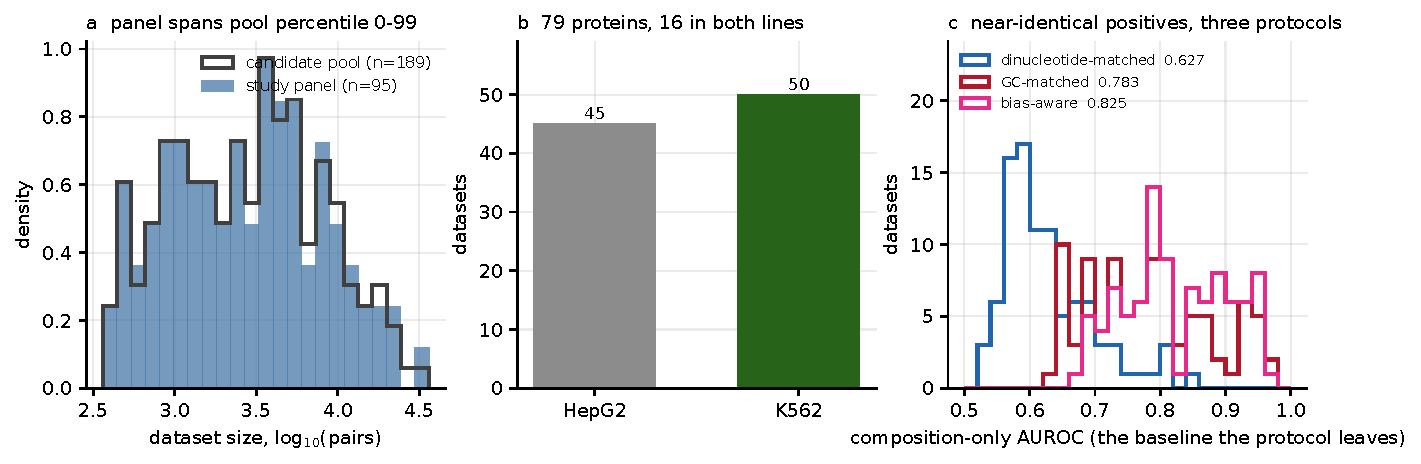
\includegraphics[width=\textwidth]{figures/f0_panel_overview.pdf}
\caption{\textbf{Study panel and size distribution.}
\textbf{(a)} Size distribution of the 94 study datasets, as $\log_{10}$ matched pairs, against
the candidate pool they were drawn from, shown as a step outline. The panel was selected as a
deterministic systematic subset by pair rank, which guarantees coverage of the size range; it is
not a probability sample and cannot be assumed free of aliasing against structure ordered by
pair count.
\textbf{(b)} Composition of the panel by protein and cell line. 79 distinct proteins, of which
15 are assayed in both K562 and HepG2 and therefore contribute two datasets each. This is why
every interval in the study resamples proteins rather than datasets.
\textbf{(c)} Composition-only AUROC under each of the three protocols, one point per dataset.
This is the independent variable of the study: the baseline each protocol leaves for a sequence
model to improve on.
\textbf{n}: 94 datasets, 79 proteins, 2 cell lines. \textbf{Uncertainty}: none plotted; panels
show distributions rather than estimates.
\textbf{Source}: \texttt{panel\_summary.csv}, \texttt{candidate\_sizes.csv},
\texttt{three\_arm\_per\_dataset.csv}.}
\end{figure}

\clearpage

% ---------------------------------------------------------------------------------------------
\begin{figure}[htbp]
\centering
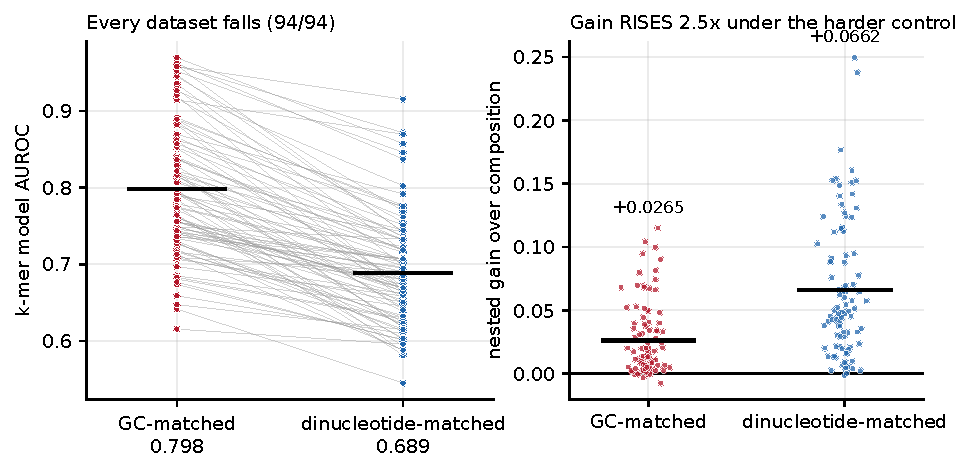
\includegraphics[width=\textwidth]{figures/f1_cost_of_matching.pdf}
\caption{\textbf{Effect of GC-matched versus dinucleotide-matched negatives on apparent AUROC
and measured contribution.}
Paired within dataset, because the two arms share nearly all of their positives; an unpaired
plot would discard the structure that makes the per-dataset counts meaningful.
\textbf{(a)} The 4-mer model's own AUROC under each protocol. It falls in every dataset, which is
expected: dinucleotide matching removes the compositional cue the model was partly using.
\textbf{(b)} The nested contribution over composition under each protocol. It rises.
The model is refitted under each protocol, and the positive sets are nearly but not perfectly
identical because each matcher rejects positives it cannot pair. Their median Jaccard similarity
is 0.9972, with exact agreement in 10 of 94 datasets.
\textbf{n}: 94 paired datasets. \textbf{Uncertainty}: not plotted; the panel-level intervals are
in the main text.
\textbf{Source}: \texttt{cost\_of\_matching.csv}.}
\end{figure}

\clearpage

% ---------------------------------------------------------------------------------------------
\begin{figure}[htbp]
\centering
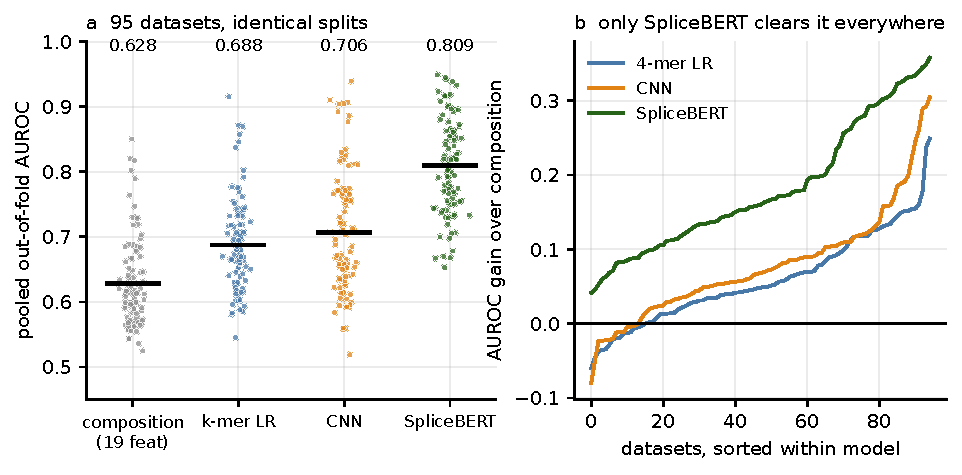
\includegraphics[width=\textwidth]{figures/f2_four_models.pdf}
\caption{\textbf{Four model classes under one protocol, on identical rows and folds.}
\textbf{(a)} Pooled out-of-fold AUROC for the 19-feature composition baseline, the 4-mer
logistic model, the convolutional network and fine-tuned SpliceBERT. Within an arm all four are
scored on the same rows under the same chromosome-grouped partition.
\textbf{(b)} The same four as a gain over the composition baseline, with datasets sorted within
each model. Only SpliceBERT exceeds the baseline in every dataset.
This methods-oriented figure establishes the performance ordering under one protocol before the
three-protocol comparison in the main text.
\textbf{n}: 94 datasets. \textbf{Uncertainty}: not plotted; each point is one dataset's pooled
out-of-fold AUROC.
\textbf{Source}: \texttt{matched\_four\_models.csv}.}
\end{figure}

\clearpage

% ---------------------------------------------------------------------------------------------
\begin{figure}[htbp]
\centering
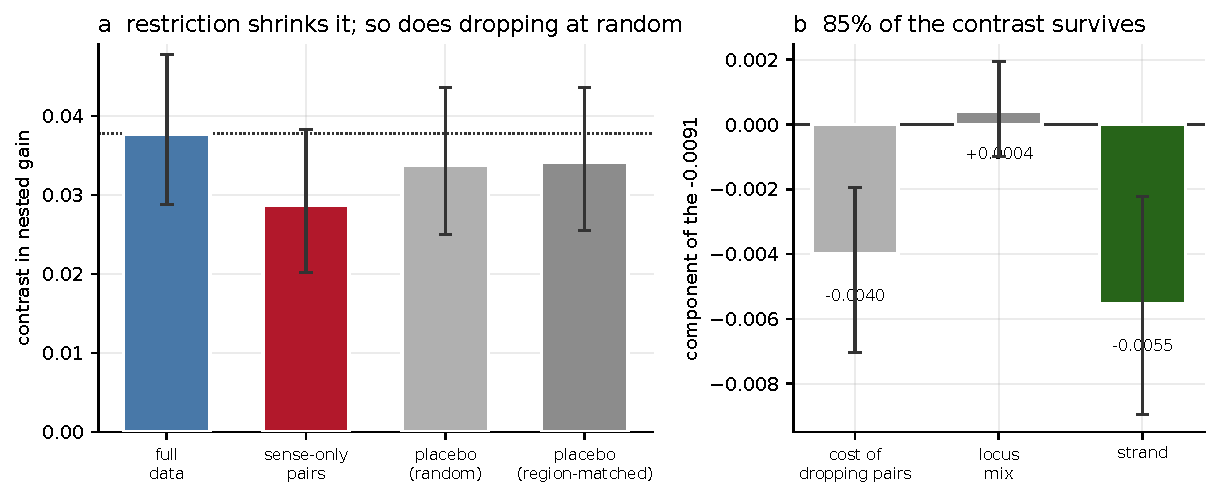
\includegraphics[width=\textwidth]{figures/f3_strand_placebo.pdf}
\caption{\textbf{Strand-control analysis.}
Negatives inherit the strand of the positive they are matched to rather than the strand of the
gene they sit in, so a fraction of them are antisense. Restricting to pairs whose negative is
unambiguously on its own gene's strand discards most of the data, and a 256-feature model loses
more from that restriction than a 19-feature baseline does, in both arms.
\textbf{(a)} The contrast under four conditions: the full data, the sense-only restriction, a
placebo dropping the same number of pairs at random, and a placebo matched on transcript region
crossed with gene-density quartile. The naive control attributes the full reduction to strand,
whereas the two placebos quantify the effect of data removal.
\textbf{(b)} The same information as a decomposition of the $-0.0091$ that restriction alone
reports, into the cost of dropping pairs at all and the strand-specific remainder.
Gene density is included because retention requires exactly one overlapping gene strand and
therefore selects against multi-gene loci by construction; the region-only placebo does not
remove that selection. The strand-specific excess is $-0.0055$, and 85.3\% of the contrast
remains after correction.
\textbf{n}: 40 datasets, over 40 distinct proteins, so protein clustering is a no-op here and is
asserted rather than assumed. 20 placebo seeds per dataset per arm.
\textbf{Uncertainty}: 95\% percentile intervals over datasets.
\textbf{Source}: \texttt{strand\_placebo.csv}.}
\end{figure}

\clearpage

% ---------------------------------------------------------------------------------------------
\begin{figure}[htbp]
\centering
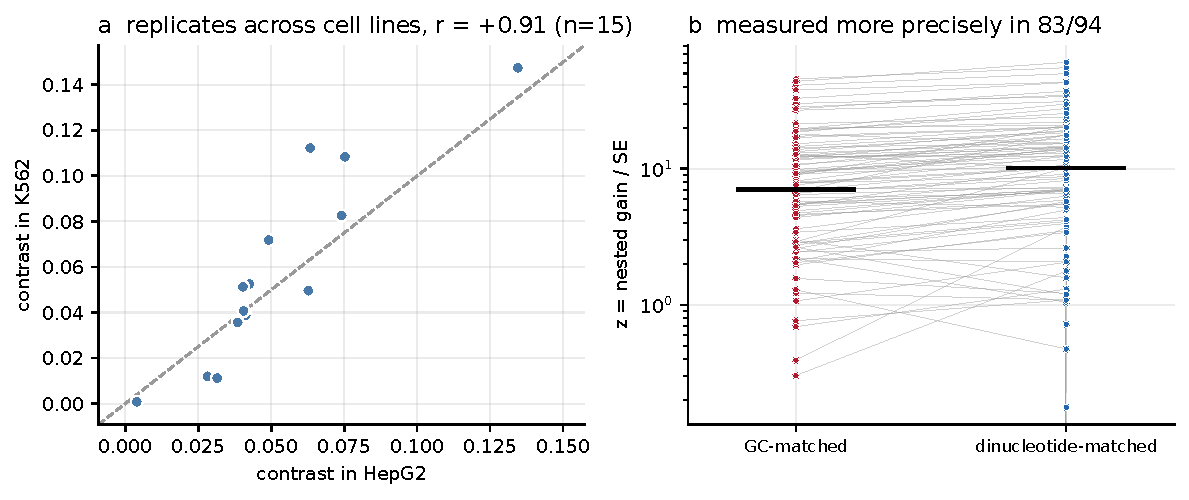
\includegraphics[width=\textwidth]{figures/f4_replication.pdf}
\caption{\textbf{The contrast replicates across cell lines, and is measured more precisely under
the harder protocol.}
\textbf{(a)} For the 15 proteins assayed in both K562 and HepG2, the contrast measured in one
cell line against the contrast measured in the other. These are separate eCLIP experiments with
separately drawn negatives, so one line is an out-of-sample prediction of the other. Pearson
$r = +0.9094$. The design forces the sign in each cell line independently and guarantees nothing
about whether the magnitudes agree, which is what makes this evidence rather than arithmetic.
\textbf{(b)} $z = \text{gain} / \text{SE}$ under each protocol, paired per dataset. The gain
rises faster than its standard error, so the same contribution reaches the same confidence with
fewer labelled windows.
After partialling out each dataset's total nested gain, the correlation is $+0.3321$ with
$p = 0.2265$, so the replication is not independent of overall signal strength.
\textbf{n}: 15 proteins for (a), 94 datasets for (b).
\textbf{Uncertainty}: Pearson correlation with a protein-level bootstrap interval in the main
text; DeLong standard errors for $z$.
\textbf{Source}: \texttt{r1\_robustness.csv}, \texttt{cost\_of\_matching.csv}.}
\end{figure}

\clearpage

% ---------------------------------------------------------------------------------------------
\begin{figure}[htbp]
\centering
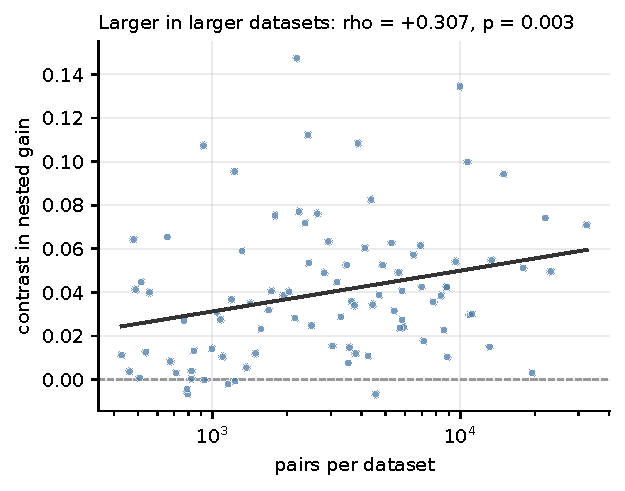
\includegraphics[width=0.62\textwidth]{figures/f5_size_modification.pdf}
\caption{\textbf{The contrast is larger in larger datasets.}
Each point is one dataset: matched pairs on a logarithmic axis against the contrast in nested
contribution between the dinucleotide-matched and GC-matched protocols.
The contrast is paired within dataset, so both arms have identical $n$ and size affects
precision rather than bias. It is reported here as effect
modification, which is a different and weaker statement: the protocol matters more where there
is more data.
\textbf{n}: 94 datasets. \textbf{Uncertainty}: Spearman correlation, printed in the panel title;
the protein-clustered interval is in the main text.
\textbf{Source}: \texttt{cost\_of\_matching.csv}, \texttt{robustness.csv}.}
\end{figure}

\clearpage

% ---------------------------------------------------------------------------------------------
\begin{figure}[htbp]
\centering
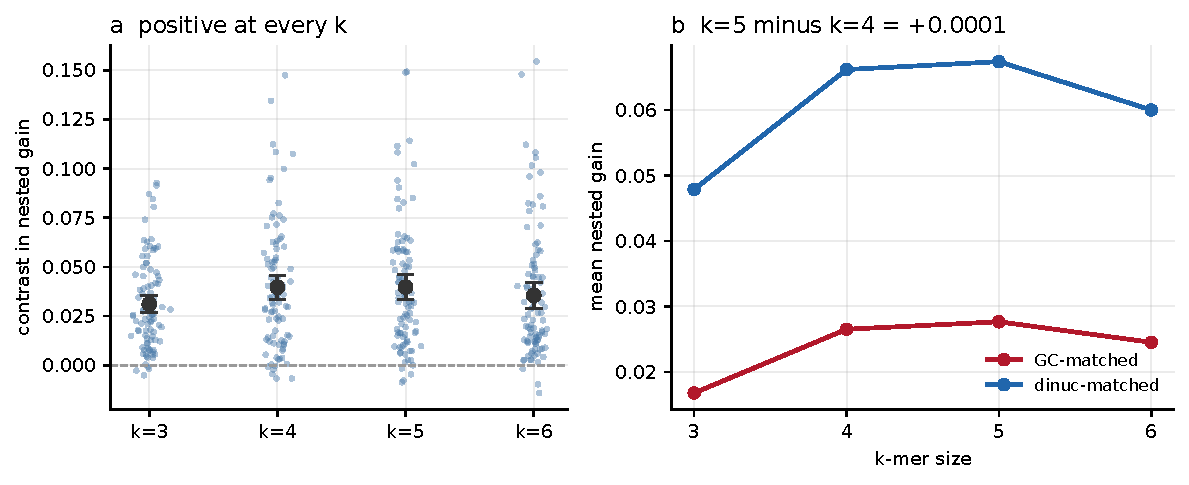
\includegraphics[width=\textwidth]{figures/f6_k_sweep.pdf}
\caption{\textbf{The contrast does not depend on the choice of $k$.}
The composition baseline and the $k$-mer model are refitted from raw sequence at four orders for
all 94 datasets in both arms, rather than read from the tables the main analysis wrote. Together
with \texttt{recompute.py} this is one of only two results in the study that are re-derived along
a different path rather than compared against a record of themselves; the rebuild reproduces the
published contrast to $1.2\times 10^{-6}$.
\textbf{(a)} The contrast at $k = 3, 4, 5, 6$, one point per dataset. Positive at every order,
and positive at every order in 82 of 94 datasets individually.
\textbf{(b)} The mean nested gain in each arm as a function of $k$, so a reader can see where the
contrast comes from rather than only its difference.
The difference between the $k=4$ and $k=5$ specifications is $+0.0001$ (paired Wilcoxon
$p = 0.84$). The contrast is also smallest at $k = 3$, so order 4 is not the most favourable
choice available.
\textbf{n}: 94 datasets per order, both arms.
\textbf{Uncertainty}: 95\% protein-clustered percentile intervals in the source table.
\textbf{Source}: \texttt{k\_sweep.csv}, \texttt{k\_sweep\_per\_dataset.csv}.}
\end{figure}

\clearpage

% ---------------------------------------------------------------------------------------------
\begin{figure}[htbp]
\centering
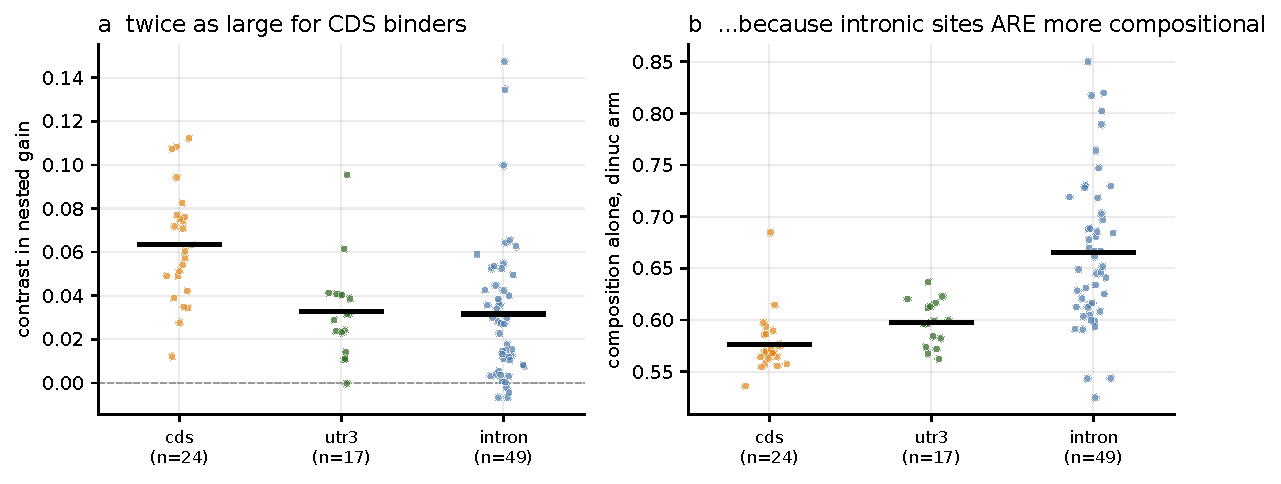
\includegraphics[width=\textwidth]{figures/f7_region.pdf}
\caption{\textbf{The contrast is larger for datasets whose binding sites are mostly coding, and
the mechanism is checkable in the same figure.}
Datasets are grouped by the transcript region their positives mostly occupy.
\textbf{(a)} The contrast by dominant region. CDS-dominant datasets give $+0.0635$ against
$+0.0316$ for intron-dominant ones, a difference of $+0.0319$, which is as large as the headline
contrast itself.
\textbf{(b)} Intronic sites are
compositionally distinctive, so composition alone already discriminates them and leaves the
protocol less to expose. Composition-only AUROC is $0.6656$ for intron-dominant datasets against
$0.5765$ for CDS-dominant ones. The intronic fraction correlates with the contrast at
$-0.3399$, but partialling out total nested gain removes the association. Region indexes how
much non-compositional signal exists; it is not an independent mechanism.
\textbf{n}: 94 datasets, grouped into three region classes with at least 8 datasets each.
\textbf{Uncertainty}: Mann--Whitney and Kruskal--Wallis tests in the source table.
\textbf{Source}: \texttt{region\_heterogeneity.csv},
\texttt{region\_heterogeneity\_per\_dataset.csv}.}
\end{figure}

\clearpage

% ---------------------------------------------------------------------------------------------
\begin{figure}[htbp]
\centering
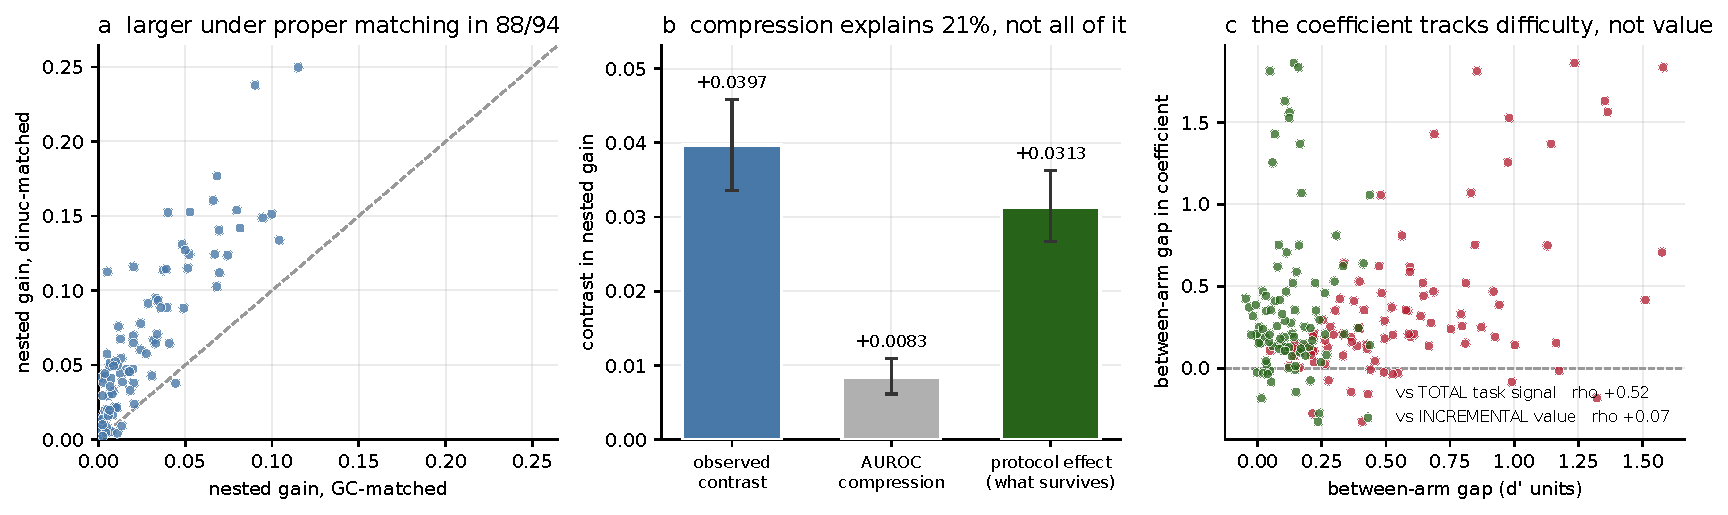
\includegraphics[width=\textwidth]{figures/f8_scale_check.pdf}
\caption{\textbf{Sensitivity of the protocol contrast to baseline compression.}
An AUROC increment is bounded above by the headroom the baseline leaves, so part of any
comparison between arms with unequal baselines is arithmetic. The transplant converts AUROC to
$d'$, moves one arm's increment onto the other arm's baseline, and asks what remains.
\textbf{(a)} The contrast per dataset, which needs no transplant and no link function: it is a
difference of two AUROC differences on the same rows.
\textbf{(b)} The transplant. Compression is real, a factor of $1.5081$, and does not account for
the contrast: the protocol effect net of scale is $+0.0313$ in one direction.
\textbf{(c)} The diagnostic behind the log-odds reversal. The between-arm coefficient gap tracks
each task's total signal rather than the incremental value it should measure, which is the
standard non-comparability of logistic coefficients across separate fits.
Running the transplant in the other direction gives $+0.0215$, and across six monotone links
and both directions the smallest member is $+0.0188$. Every member keeps the sign, so the
contrast is not a compression artefact. The range of estimates supports treating the
decomposition as a sensitivity analysis. Separately, the
identifying assumption that the $d'$ increment is baseline-invariant is refuted by its own
diagnostic, so no model's protocol effect is point-identified.
\textbf{n}: 94 datasets. \textbf{Uncertainty}: 95\% protein-clustered percentile intervals.
\textbf{Source}: \texttt{scale\_check.csv}, \texttt{protocol\_identification.csv}.}
\end{figure}

\clearpage

% ---------------------------------------------------------------------------------------------
\begin{figure}[htbp]
\centering
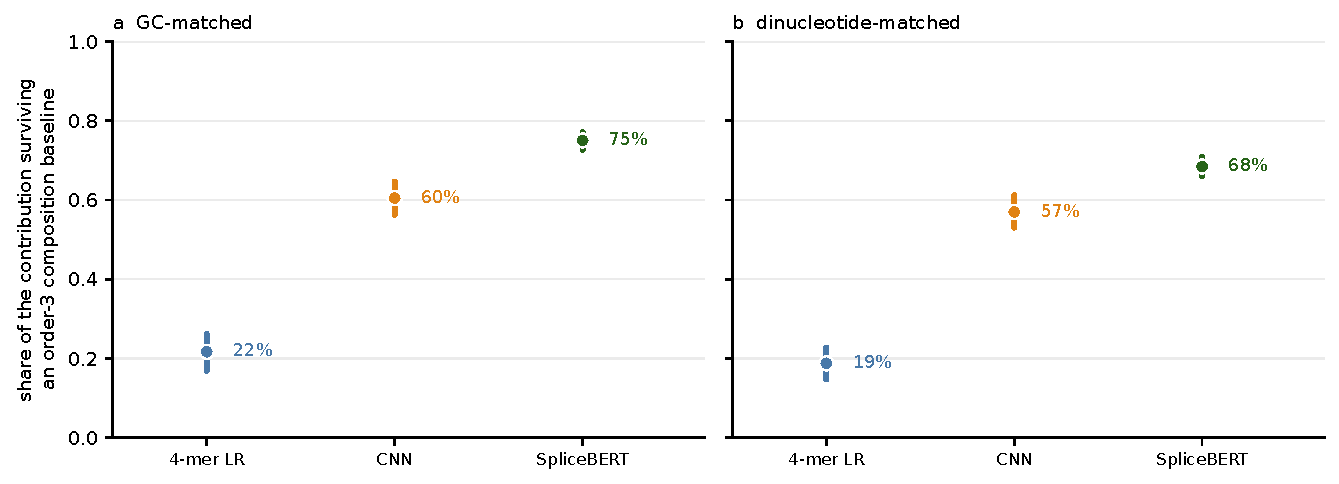
\includegraphics[width=\textwidth]{figures/f13_baseline_order_models.pdf}
\caption{\textbf{Raising the composition baseline from order 2 to order 3, for all three model
classes.}
The composition baseline stops at dinucleotides while the headline model is a 4-mer, so the
measured quantity is short-range compositional signal one order above wherever the matcher
stopped. Where the baseline stops is an analyst's choice, and this figure measures what that
choice costs. The extended baseline adds all 64 trinucleotide frequencies, 82 features in total.
\textbf{(a)} GC-matched arm and \textbf{(b)} dinucleotide-matched arm: the share of each model's
contribution that survives an order-3 baseline. For the 4-mer the surviving share on the GC arm
is $0.2170$, against $0.6049$ for the convolutional network and $0.7504$ for SpliceBERT.
The \emph{absolute} amount absorbed is statistically indistinguishable across model
classes, and the convolutional network loses the least of the three, which no capacity story
predicts. The shares follow from the totals. What the figure supports is that the protocol
contrast survives an order-3 baseline for every model class, not that the 4-mer is uniquely
fragile.
\textbf{n}: 94 datasets, three model classes, two arms.
\textbf{Uncertainty}: 95\% protein-clustered percentile intervals in the source table.
\textbf{Source}: \texttt{baseline\_order\_models.csv},
\texttt{baseline\_order\_models\_per\_dataset.csv}.}
\end{figure}

\clearpage

% ---------------------------------------------------------------------------------------------
\section*{Table S1. Dataset to ENCODE accession}

The table below is typeset from \texttt{supplementary\_table\_s1.csv}, which ships beside this
document and is committed under \texttt{results/}\allowbreak\texttt{tables/}. The CSV carries
six further columns, each arm's composition baseline and contribution, which do not fit a
portrait page; the accession mapping is reproduced here so that this document is readable on its
own.

One row has the three-arm flag false: NCBP2 in K562 cleared the minimum-pair floor under
dinucleotide matching and not under GC matching, so it is in the candidate panel and has no
three-protocol result. That is the difference between the 95 selected datasets and the 94 the
study reports on.

% GENERATED by scripts/table_s1_tex.py from results/tables/supplementary_table_s1.csv.
% Do not edit: build.sh regenerates it, so an edit here is silently discarded.
\begin{longtable}{llllrrc}
\caption{\textbf{Dataset to ENCODE accession.} All 95 datasets in the candidate panel, one row each, with the ENCODE file and experiment accessions needed to retrieve the source peaks. \textbf{3 arms} is whether the dataset carries all three negative-set protocols; the 1 marked \textit{no} cleared the minimum-pair floor under dinucleotide matching but not under GC matching, which is the difference between the 95 selected datasets and the 94 the study reports on. The same table with each arm's composition baseline and contribution is \texttt{supplementary\_table\_s1.csv}, which ships beside this document.}\label{tab:s1}\\
\toprule
\textbf{protein} & \textbf{cell line} & \textbf{ENCFF file} & \textbf{ENCSR experiment} & \textbf{reps} & \textbf{pairs} & \textbf{3 arms} \\
\midrule
\endfirsthead
\multicolumn{7}{l}{\textit{Table S1, continued}}\\
\toprule
\textbf{protein} & \textbf{cell line} & \textbf{ENCFF file} & \textbf{ENCSR experiment} & \textbf{reps} & \textbf{pairs} & \textbf{3 arms} \\
\midrule
\endhead
\midrule\multicolumn{7}{r}{\textit{continued on the next page}}\\
\endfoot
\bottomrule
\endlastfoot
AATF & K562 & ENCFF955LYD & ENCSR819XBT & 2 & 1{,}081 & yes \\
AKAP1 & HepG2 & ENCFF749IUB & ENCSR356ZMO & 2 & 5{,}943 & yes \\
AQR & HepG2 & ENCFF323PUC & ENCSR018WPY & 2 & 11{,}101 & yes \\
BCCIP & HepG2 & ENCFF134LIU & ENCSR485QCG & 2 & 539 & yes \\
BCLAF1 & HepG2 & ENCFF810EUA & ENCSR876EYA & 2 & 32{,}387 & yes \\
BUD13 & K562 & ENCFF262ILV & ENCSR663WES & 2 & 8{,}850 & yes \\
CDC40 & HepG2 & ENCFF027MEO & ENCSR815VVI & 2 & 1{,}172 & yes \\
CSTF2T & HepG2 & ENCFF141DOI & ENCSR919HSE & 2 & 18{,}864 & yes \\
DDX24 & K562 & ENCFF537KWB & ENCSR999WKT & 2 & 9{,}600 & yes \\
DDX55 & HepG2 & ENCFF797QRS & ENCSR845VGB & 2 & 1{,}686 & yes \\
DDX55 & K562 & ENCFF462WAI & ENCSR923NKN & 2 & 1{,}101 & yes \\
DDX59 & HepG2 & ENCFF899AWZ & ENCSR214BZA & 2 & 3{,}089 & yes \\
DDX6 & HepG2 & ENCFF614NUP & ENCSR141OIM & 2 & 493 & yes \\
DDX6 & K562 & ENCFF904KTV & ENCSR893EFU & 2 & 1{,}955 & yes \\
DGCR8 & K562 & ENCFF023YVD & ENCSR947JVR & 2 & 1{,}253 & yes \\
DHX30 & K562 & ENCFF128AKC & ENCSR529GSJ & 2 & 824 & yes \\
DROSHA & HepG2 & ENCFF854BHP & ENCSR834YLD & 2 & 2{,}184 & yes \\
DROSHA & K562 & ENCFF797BHU & ENCSR653HQC & 2 & 3{,}915 & yes \\
EFTUD2 & HepG2 & ENCFF796RMF & ENCSR527DXF & 2 & 7{,}401 & yes \\
EIF3H & HepG2 & ENCFF813JIK & ENCSR916XIV & 2 & 2{,}832 & yes \\
ELAC2 & K562 & ENCFF850ZSC & ENCSR440MSY & 2 & 12{,}915 & yes \\
ELAVL1 & K562 & ENCFF566LNK & ENCSR090LNQ & 2 & 8{,}806 & yes \\
EXOSC5 & HepG2 & ENCFF862EKD & ENCSR693JWP & 2 & 727 & yes \\
FASTKD2 & HepG2 & ENCFF498IGK & ENCSR023UHL & 2 & 868 & yes \\
FASTKD2 & K562 & ENCFF423SOR & ENCSR887FHF & 2 & 542 & yes \\
FKBP4 & HepG2 & ENCFF957AOZ & ENCSR018ZUE & 2 & 1{,}454 & yes \\
FMR1 & K562 & ENCFF630KXK & ENCSR554UVB & 2 & 4{,}445 & yes \\
FXR1 & K562 & ENCFF366UJP & ENCSR774RFN & 2 & 1{,}425 & yes \\
FXR2 & K562 & ENCFF111LMZ & ENCSR767OEY & 2 & 4{,}745 & yes \\
G3BP1 & HepG2 & ENCFF899HHP & ENCSR721HPX & 2 & 6{,}482 & yes \\
GARS & K562 & ENCFF390NMJ & ENCSR448GXJ & 2 & 566 & yes \\
GEMIN5 & K562 & ENCFF050VVI & ENCSR238CLX & 2 & 2{,}640 & yes \\
GRSF1 & HepG2 & ENCFF929AWR & ENCSR668MJX & 2 & 1{,}008 & yes \\
GRWD1 & HepG2 & ENCFF159MMZ & ENCSR893NWB & 2 & 22{,}078 & yes \\
GRWD1 & K562 & ENCFF327DLL & ENCSR999YGP & 2 & 4{,}375 & yes \\
GTF2F1 & HepG2 & ENCFF002HYO & ENCSR265ZIS & 2 & 4{,}472 & yes \\
HLTF & HepG2 & ENCFF048FDF & ENCSR647HOX & 2 & 3{,}645 & yes \\
HNRNPC & K562 & ENCFF167CDB & ENCSR249ROI & 2 & 516 & yes \\
HNRNPL & K562 & ENCFF917CBK & ENCSR795CAI & 2 & 5{,}840 & yes \\
HNRNPM & HepG2 & ENCFF752JNY & ENCSR267UCX & 2 & 13{,}423 & yes \\
HNRNPUL1 & HepG2 & ENCFF610JVZ & ENCSR755TJC & 2 & 467 & yes \\
IGF2BP1 & K562 & ENCFF650LMV & ENCSR975KIR & 2 & 5{,}706 & yes \\
KHSRP & HepG2 & ENCFF771QAU & ENCSR366DGX & 2 & 5{,}289 & yes \\
KHSRP & K562 & ENCFF031FMO & ENCSR438GZQ & 2 & 23{,}190 & yes \\
LARP4 & HepG2 & ENCFF534JCV & ENCSR805SRN & 2 & 5{,}429 & yes \\
LARP4 & K562 & ENCFF947CIN & ENCSR888YTT & 2 & 430 & yes \\
LIN28B & K562 & ENCFF061XNA & ENCSR970NKP & 2 & 6{,}916 & yes \\
LSM11 & K562 & ENCFF858EHN & ENCSR022BVV & 2 & 1{,}339 & yes \\
MATR3 & HepG2 & ENCFF587KKM & ENCSR290VLT & 2 & 6{,}991 & yes \\
MATR3 & K562 & ENCFF246EPM & ENCSR440SUX & 2 & 4{,}866 & yes \\
MBNL1 & K562 & ENCFF603WDI & ENCSR497XZI & 2 & 1{,}202 & yes \\
METTL1 & K562 & ENCFF125IDN & ENCSR498DQS & 2 & 481 & yes \\
MORC2 & K562 & ENCFF605AFN & ENCSR168VUE & 2 & 891 & yes \\
MTPAP & K562 & ENCFF883KCN & ENCSR200DKE & 2 & 1{,}083 & yes \\
NCBP2 & HepG2 & ENCFF692RZM & ENCSR018RVZ & 2 & 3{,}226 & yes \\
NCBP2 & K562 & ENCFF886MLH & ENCSR484LTQ & 2 & 406 & no \\
NKRF & HepG2 & ENCFF045HSV & ENCSR277DEO & 2 & 3{,}794 & yes \\
NOLC1 & K562 & ENCFF327YTD & ENCSR001VAC & 2 & 1{,}570 & yes \\
NONO & K562 & ENCFF730QRI & ENCSR861PAR & 2 & 11{,}333 & yes \\
PCBP1 & HepG2 & ENCFF098REE & ENCSR256CHX & 2 & 940 & yes \\
PCBP2 & HepG2 & ENCFF642GNE & ENCSR339FUY & 2 & 8{,}526 & yes \\
PHF6 & K562 & ENCFF588ITW & ENCSR001KKZ & 2 & 695 & yes \\
PPIL4 & K562 & ENCFF559HGK & ENCSR197INS & 2 & 659 & yes \\
PRPF4 & HepG2 & ENCFF227EJF & ENCSR977OXG & 2 & 9{,}159 & yes \\
PTBP1 & HepG2 & ENCFF726SQU & ENCSR384KAN & 2 & 7{,}988 & yes \\
PTBP1 & K562 & ENCFF907HNN & ENCSR981WKN & 2 & 7{,}608 & yes \\
PUM1 & K562 & ENCFF094MQV & ENCSR308YNT & 2 & 2{,}658 & yes \\
QKI & HepG2 & ENCFF704OCI & ENCSR570WLM & 2 & 9{,}990 & yes \\
QKI & K562 & ENCFF786UOW & ENCSR366YOG & 2 & 2{,}189 & yes \\
RBFOX2 & K562 & ENCFF206RIM & ENCSR756CKJ & 2 & 3{,}519 & yes \\
RBM15 & HepG2 & ENCFF054VLU & ENCSR754NDA & 2 & 1{,}500 & yes \\
RPS3 & HepG2 & ENCFF301IJW & ENCSR766FAC & 2 & 5{,}658 & yes \\
RPS3 & K562 & ENCFF530HTL & ENCSR120EAR & 2 & 2{,}372 & yes \\
SAFB2 & K562 & ENCFF594EDV & ENCSR943MHU & 2 & 3{,}744 & yes \\
SLTM & K562 & ENCFF696QWE & ENCSR000SSH & 2 & 3{,}640 & yes \\
SMNDC1 & K562 & ENCFF943XOU & ENCSR658IQB & 2 & 2{,}465 & yes \\
SND1 & K562 & ENCFF211TRO & ENCSR128VXC & 2 & 4{,}132 & yes \\
SRSF1 & HepG2 & ENCFF934ANS & ENCSR989VIY & 2 & 1{,}791 & yes \\
SRSF1 & K562 & ENCFF223KVR & ENCSR321PWZ & 2 & 3{,}864 & yes \\
STAU2 & HepG2 & ENCFF678FCX & ENCSR979EWD & 2 & 848 & yes \\
SUB1 & HepG2 & ENCFF335JTC & ENCSR406OOZ & 2 & 3{,}297 & yes \\
TAF15 & HepG2 & ENCFF566EAE & ENCSR841EQA & 2 & 768 & yes \\
TIA1 & HepG2 & ENCFF759KCD & ENCSR623VEQ & 2 & 1{,}729 & yes \\
TIA1 & K562 & ENCFF918KMT & ENCSR057DWB & 2 & 5{,}883 & yes \\
TRA2A & HepG2 & ENCFF766OCH & ENCSR314UMJ & 2 & 921 & yes \\
U2AF1 & K562 & ENCFF640IHY & ENCSR862QCH & 2 & 1{,}230 & yes \\
U2AF2 & HepG2 & ENCFF721PWF & ENCSR202BFN & 2 & 10{,}702 & yes \\
UCHL5 & HepG2 & ENCFF573DXD & ENCSR490IEE & 2 & 2{,}233 & yes \\
XPO5 & HepG2 & ENCFF327VCE & ENCSR921SXC & 2 & 4{,}615 & yes \\
YBX3 & HepG2 & ENCFF185OEI & ENCSR735HOK & 2 & 2{,}042 & yes \\
YBX3 & K562 & ENCFF746XLE & ENCSR529FKI & 2 & 17{,}979 & yes \\
YWHAG & K562 & ENCFF932UXC & ENCSR867ZVK & 2 & 798 & yes \\
ZNF622 & K562 & ENCFF285IGP & ENCSR657TZZ & 2 & 14{,}969 & yes \\
ZNF800 & HepG2 & ENCFF343TCO & ENCSR685AUR & 2 & 2{,}938 & yes \\
ZNF800 & K562 & ENCFF105HMJ & ENCSR586DGV & 2 & 2{,}436 & yes \\
\end{longtable}


\end{document}
